\chapter{Tabelle disequazioni}
\label{cha:TabelleDisisequazionia}
\begin{sidewaysfigure}
	\begin{subfigure}[b]{.5\linewidth}
		\centering
\includestandalone[width=\textwidth]{quarto/DisSecGrado/DeltaMaggioreDiZeroAmaggioreDizero}
		\caption{$\Delta>0$ $a>0$}\label{graf:dis2GDeltaMagZa2xa}
	\end{subfigure}%
\quad
	\begin{subfigure}[b]{.5\linewidth}
		\centering
	\includestandalone[width=\textwidth]{quarto/DisSecGrado/DeltaMaggioreDiZeroAminoreDizero}
		\caption{$\Delta>0$ $a<0$}\label{graf:dis2GDeltaMagZb2xa}
	\end{subfigure}
\vskip .8cm
	\begin{subfigure}[b]{.5\linewidth}
		\centering
		\includestandalone[width=\textwidth]{quarto/DisSecGrado/DeltaUgualeaZeroAmaggioreDizero}
		\caption{$\Delta=0$ $a>0$}\label{graf:dis2GDeltaUguaZa2xa}
			\end{subfigure}%
\quad
	\begin{subfigure}[b]{.5\linewidth}
		\centering
		\includestandalone[width=\textwidth]{quarto/DisSecGrado/DeltaUgualeaZeroAminoreDizero}
		\caption{$\Delta=0$ $a<0$}\label{graf:dis2GDeltaUguaZb2xa}
	\end{subfigure}
\vskip .8cm
\begin{subfigure}[b]{.5\linewidth}
	\centering
		\includestandalone[width=\textwidth]{quarto/DisSecGrado/DeltaMinoreZeroAmaggioreDizero}
	\caption{$\Delta<0$ $a>0$}\label{graf:dis2GDeltaMinorZa2xa}
\end{subfigure}%
\quad
\begin{subfigure}[b]{.5\linewidth}
	\centering
\includestandalone[width=\textwidth]{quarto/DisSecGrado/DeltaMinoreZeroAminoreDizero}
	\caption{$\Delta<0$ $a<0$}\label{graf:dis2GDeltaMinorZb2xa}
\end{subfigure}
	\caption{Grafici disequazione di secondo grado}
\end{sidewaysfigure}
\begin{sidewaystable}
	\centering
	\begin{tabular}{@{}m{1cm}m{11cm}m{11cm}}
	%	\toprule
		& \centering $a>0$ & \centering$a<0$ \tabularnewline
\centering$\Delta>0$ &\tabincludestandalone[width=10.5cm]{quarto/DisSecGrado/DeltaMaggioreDiZeroAmaggioreDizero}  & \vskip .8cm 	\tabincludestandalone[width=10.5cm]{quarto/DisSecGrado/DeltaMaggioreDiZeroAminoreDizero} \\[1cm] 
		\centering$\Delta=0$ & 	\tabincludestandalone[width=10.5cm]{quarto/DisSecGrado/DeltaUgualeaZeroAmaggioreDizero} &\vskip .5cm   \tabincludestandalone[width=10.5cm]{quarto/DisSecGrado/DeltaUgualeaZeroAminoreDizero}\\[1cm] 
		\centering$\Delta<0$ & \tabincludestandalone[width=10.5cm]{quarto/DisSecGrado/DeltaMinoreZeroAmaggioreDizero} &\vskip .5cm  \tabincludestandalone[width=10.5cm]{quarto/DisSecGrado/DeltaMinoreZeroAminoreDizero}\\[1cm] 
	%	\bottomrule
	\end{tabular}
	\caption{Segno disequazioni secondo grado}
\end{sidewaystable}
\begin{table}
	\centering
	\begin{tikzpicture}
	\tkzTabInit[color,lgt=5,espcl=3]%
	{$x$ / .8,$\Delta>0$\\ Il segno di\\ $ax^2+bx+c$ /2}%
	{$-\infty$,$x_1$,$x_2$,$+\infty$}%
	\tkzTabLine{ , \genfrac{}{}{0pt}{0}{\text{segno di}}{a}, z
		, \genfrac{}{}{0pt}{0}{\text{segno}}{\text{opposto di}\ a}, z
		, \genfrac{}{}{0pt}{0}{\text{segno di}}{a}, }
	\end{tikzpicture}\\
	\begin{tikzpicture}
	\tkzTabInit[color,lgt=5,espcl=3]%
	{$x$ / .8, $\Delta=0$\\ Il segno di\\ $ax^2+bx+c$ / 2}%
	{$-\infty$,$x_1$,$+\infty$}%
	\tkzTabLine{ , \genfrac{}{}{0pt}{0}{\text{segno di}}{ a} , z
		, \genfrac{}{}{0pt}{0}{\text{segno di}}{a}, }
	\end{tikzpicture}\\
	\begin{tikzpicture}
	\tkzTabInit[color,lgt=5,espcl=5]%
	{$x$/.8,$\Delta<0$\\ Il segno di\\ $ax^2+bx+c$/2}%
	{$-\infty$,$+\infty$}%
	\tkzTabLine{ , \genfrac{}{}{0pt}{0}{\text{segno di}}{ a}, }
	\end{tikzpicture}
	\caption{Segno disequazione di secondo grado}
	\label{tab:segnodisequazioni2gradoa}
\end{table}
\begin{sidewaystable}
	\centering
\begin{tabular}{@{}cc>{\centering}m{10.5cm}>{\centering}m{10.5cm}}
	&  & $a>0$ &  $a<0$ \tabularnewline[0.5cm] 
	&  & 	\tabincludestandalone[width=10.5cm]{quarto/DisSecGrado/DeltaMaggioreDiZeroAmaggioreDizero}  & 	\tabincludestandalone[width=10.5cm]{quarto/DisSecGrado/DeltaMaggioreDiZeroAminoreDizero} \tabularnewline[0.5cm] 
	\multirow{4}{1cm}{$\Delta>0$}	& $ax^2+bx+c\geq 0$ & $x\leq x_1$ e $x\geq x_2$  & $x_1\leq x \leq x_2$ \tabularnewline  
	& $ax^2+bx+c > 0$ &$x< x_1$ e $x>x_2$  & $x_1< x < x_2$ \tabularnewline
	& $ax^2+bx+c\leq 0$ & $x_1\leq x \leq x_2$ & $x\leq x_1$ e $x\geq x_2$ \tabularnewline  
	& $ax^2+bx+c< 0$ & $x_1< x < x_2$ & $x< x_1$ e $x>x_2$ \tabularnewline
	&\tabularnewline
	&  & 	\tabincludestandalone[width=10.5cm]{quarto/DisSecGrado/DeltaUgualeaZeroAmaggioreDizero} &  \tabincludestandalone[width=10.5cm]{quarto/DisSecGrado/DeltaUgualeaZeroAminoreDizero}\tabularnewline[0.5cm] 
	\multirow{4}{1cm}{$\Delta=0$}	& $ax^2+bx+c\geq 0$ & Sempre & $x=x_1$ \tabularnewline  
	& $ax^2+bx+c > 0$ & Sempre $x\neq x_1$ & Mai \tabularnewline
	& $ax^2+bx+c\leq 0$ & $x=x_1 $  & Sempre \tabularnewline  
	& $ax^2+bx+c< 0$ & Mai & Sempre $x\neq x_1$ \tabularnewline  
		&\tabularnewline
	&  & 	\tabincludestandalone[width=10.5cm]{quarto/DisSecGrado/DeltaMinoreZeroAmaggioreDizero} & \tabincludestandalone[width=10.5cm]{quarto/DisSecGrado/DeltaMinoreZeroAminoreDizero}\tabularnewline[0.5cm] 
	\multirow{4}{1cm}{$\Delta<0$}	& $ax^2+bx+c\geq 0$ & Sempre. Uguale a zero mai & Mai \tabularnewline  
	& $ax^2+bx+c > 0$ & Sempre & Mai \tabularnewline
	& $ax^2+bx+c\leq 0$ & Mai & Sempre. Uguale a zero mai \tabularnewline  
	& $ax^2+bx+c< 0$ & Mai & Sempre \tabularnewline  
\end{tabular} 
\end{sidewaystable}
 
	
